% ...................................................................
\chapter{Finite Elements Method}
\section{Description of a Finite Element}

\subsection{Formal definition of a Finite Element}

Let $(K,P,\Sigma)$ be a triple such that

(i) $K$ is a closed subset of $\ \mathbb{R}^n$ of non empty interior,

(ii) $P$ is a finite dimensional vector space of functions defined on $K$,

(iii) $\Sigma$ is a set of linear forms on $P$ of finite cardinal
 $N$, $\Sigma=\{\sigma_1,\dots,\sigma_N\}$.

\begin{definition}
The elements of $\Sigma$ are called \emph{degrees of freedom} of the Finite Element.
\end{definition}
The degrees of freedom characterise the basis of $P$ associated to the Finite Element.

\begin{definition} 
  $\Sigma$ is said to be \textbf{$P$-unisolvent} if for any $N$-tuple
$(\alpha_1,\dots,\alpha_N)$, there  exists a unique element $p\in P$ such that
$\sigma_i(p)=\alpha_i$ pour $i=1,\dots, N$.
\end{definition} 
\begin{definition}
  The triple $(K,P,\Sigma)$ of $ \mathbb{R}^n$ is called \textbf{Finite Element} of $ \mathbb{R}^n$ if it satisfies
     (i), (ii) and (iii) and if $\Sigma$
  is $P$-unisolvent.
\end{definition}

In the definition of a Finite Element, $K$ is the domain on which the Finite Element is defined, $P$ is the finite dimensional approximation space, and $\Sigma$ uniquely defines a basis of $P$, which is needed to build the Finite Element matrices associated to the variational formulation applied to functions in the Finite Dimensional approximation space. This basis can be either defined through the degrees of freedom or directly by exhibiting an explicit formula for the basis functions. In this last case the degrees of freedom are not explicitly needed. 

The unisolvence property is needed to establish that the elements of $P$ characterised by the degrees fo freedom actually form a basis of $P$. In practice, this is done by first verifying that the dimension is right, \textit{i.e.} that the number of degrees of freedom is equal to $\dim P=N$ and then by checking either the injectivity or the surjectivity, which both imply the bijectivity if the dimension is right, of the mapping
\begin{align*}
P &\rightarrow \mathbb{R}^N\\
p &\mapsto (\sigma_1(p), \dots,  \sigma_N(p))
\end{align*}
This can be formalised in the two following lemmas:
\begin{lemma}\label{lemma:unisolvInj}
The set $\Sigma$ is $P$-unisolvent if and only if the two following properties are satisfied
\begin{itemize}
\item[(i)] $\dim P = |\Sigma|$ (where $|\Sigma|$ denotes the number of elements in the set $\Sigma$).
\item[(ii)] $\sigma_j(p)=0$ for $j=1, \dots, N$ $\Rightarrow p=0$.
\end{itemize}
\end{lemma}

\begin{lemma}\label{lemma:unisolvSurj}
The set $\Sigma$ is $P$-unisolvent if and only if the two following properties are satisfied
\begin{itemize}
\item[(i)] $\dim P = |\Sigma|=N$.
\item[(ii)] There exist $N$ linearly independent functions $p_i\in P, \,i=1, \dots, N$ such that $\sigma_j(p_i)=\delta_{ij}$.
\end{itemize}
\end{lemma}

In addition to its local definition, independent of its neighbours, the degrees of freedom of a Finite Element need to be chosen to allow a natural embedding into the function spaces in which the variational formulation is defined.
In practice for Finite Element spaces embedded in $L^2$ no continuity is required,   for Finite Element spaces embedded in $H^1$ $C^0$ continuity is required, for Finite Element spaces embedded in $H^2$ $C^1$ continuity is required, for Finite Element spaces embedded in $ H(\textrm{curl}, \Omega) $ $C^0$ continuity of the tangential component is required and for Finite Element spaces embedded in $ H(\textrm{div}, \Omega) $ $C^0$ continuity of the normal component is required. 

We will thus present examples of Finite Elements according to their conformity, \textit{i.e.} to the space in which they can be naturally embedded. Note that the continuity requirement is enforced by sharing the degrees of freedom on the interface between two elements and by making sure that these define uniquely the trace of $P$ on the interface.

\begin{remark}
Note that not all degrees of freedom on the interface need to be shared between the elements sharing the interface. This needs to be decided when constructing the global Finite Element space from the reference element.
\end{remark}

\subsection{$C^0$ Lagrange Finite Elements}

These are continuous Finite Elements, and the continuity will be enforced by sharing the degrees of freedom on the interface.   Thanks to this continuity property the Finite Element constructed from those will be included in $H^1$. These elements are called \emph{$H^1$ conforming}.

\paragraph{1D Lagrange $\mathbb{P}_k$ Element } Let $a,b\in \mathbb{R}$, $a<b$. Let $K=[a,b]$, 
$P= \mathbb{P}_k$ the set of polynomials of degree $k$ on $[a,b]$, $\Sigma=\{\sigma_0, \dots,
\sigma_k\}$, where $a= x_0 < x_1 < \dots < x_k= b$ are distinct points and
$$
\begin{array}{rcl}
\sigma_k:P&\rightarrow & \mathbb{R},\\
p&\mapsto &p(x_i).
\end{array}$$
Moreover $\Sigma$ is $P$-unisolvant, using Lemma \ref{lemma:unisolvSurj}. Indeed the Lagrange polynomials
at the interpolation points $x_0,x_1, \dots, x_k$ which read
\begin{equation}\label{eq:LagrangePol}
l_{k,i}(x)=\frac{\displaystyle \prod_{\substack{0\leq j\leq k \\ j\neq i}} (x -x_j)}{
\displaystyle \prod_{\substack{0\leq j\leq k \\ j\neq i}} (x_i -x_j)}
\end{equation}
satisfy 
 $l_{k,i}(x_j)=\delta_{i,j}$, $0\leq i,j \leq k$.
 
The fact that the  points  are all distinct makes the Lagrange interpolation problem well posed. The first and last point being on the boundary, will correspond to shared degrees of freedom. The corresponding basis function will be shared with the neighbouring element.

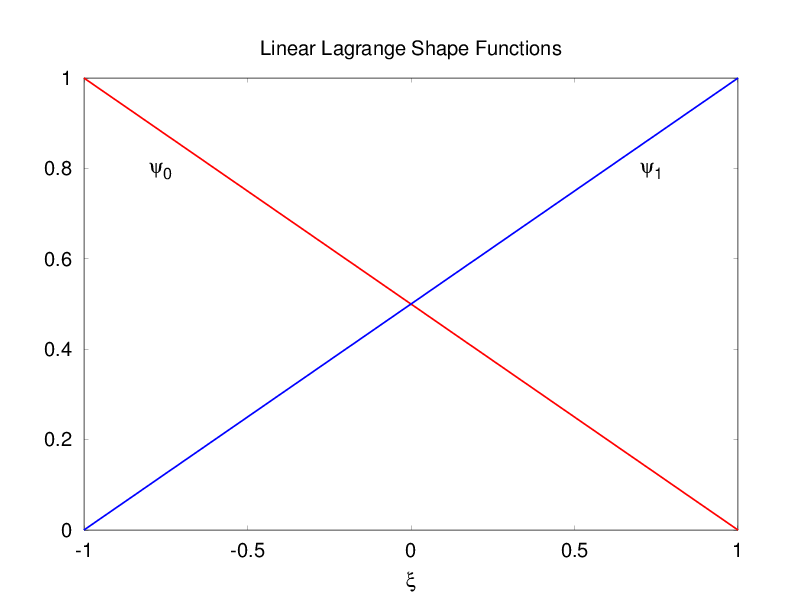
\includegraphics[width=.3\textwidth]{figures/part_4/linear_lagrange}
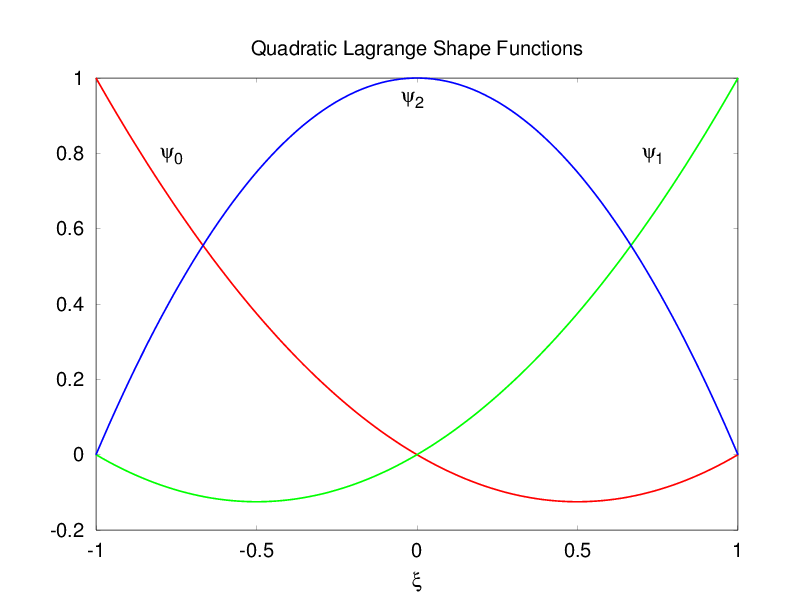
\includegraphics[width=.3\textwidth]{figures/part_4/quadratic_lagrange}
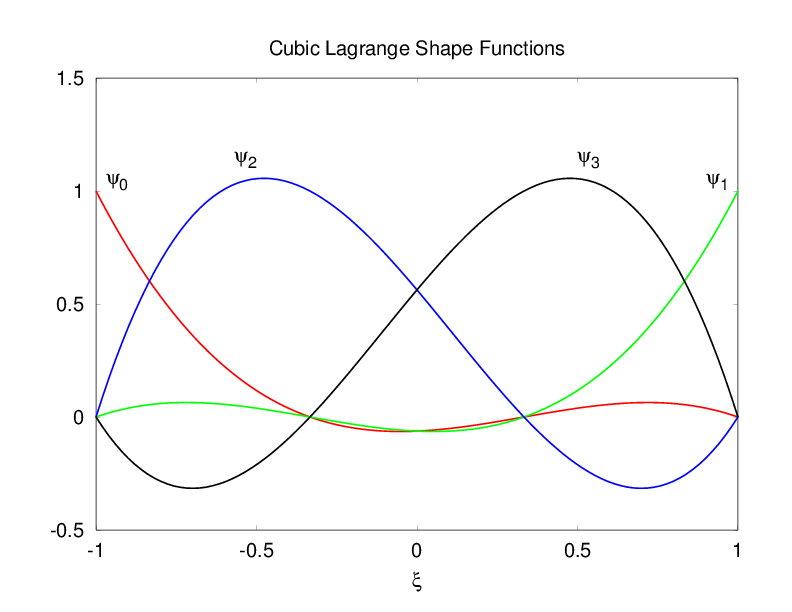
\includegraphics[width=.3\textwidth]{figures/part_4/cubic_lagrange}
 
For low degree polynomials, typically up to three, the degrees of freedom can be chosen uniformly space. For higher degree, the resulting matrices have better properties in particular conditioning if Gauss-Lobatto points are chosen. Note that high order Lagrange Finite Elements based on Gauss-Lobatto points are often called \emph{spectral elements}.

The extension from one to multiple dimensions is generally done in two ways. Either one builds finite elements based on simplices, or on tensor products of 1D elements. There are other possibilities but they are less classical. 

\paragraph{Simplex based $ \mathbb{P}_k$ Finite Elements.}
A simplex in $n$ dimensions is the convex hull of $n+1$ affine independent points. In 2D this is a non degenerate triangle in 3D a tetrahedron. In simplices basis functions are most easily expressed using the barycentric coordinates associated to the vertices of the simplex, that we shall denote by $ \mathbf{a}_0, \dots, \mathbf{a}_n \in \mathbb{R}^n$. The barycentric coordinate, classically denoted by $(\lambda_i)_{0\leq i\leq n}$, associated to the vertex $ \mathbf{a}_i$ is the affine function with value 1 at $ \mathbf{a}_i$ and 0 at the $n$ other vertices. More precisely, for any point $ \mathbf{x}=(x_1,\dots,x_n)^\top \in \mathbb{R}^{n}$,
\begin{equation}\label{eq:barcoord}
\lambda_i( \mathbf{x}) = \alpha_{i,0} + \sum_{l=1}^n \alpha_{i,l} x_l, ~~~ i=0,\dots,n.
\end{equation}
The coefficients $(\alpha_{i,l})_{0\leq l \leq n}$ being determined by the relations  $\lambda_i( \mathbf{a}_j)  =\delta_{ij}$.

\textit{Example: $\mathbb{P}_k$ in 2D.} For 3 non aligned points $ \mathbf{a}_1$, $ \mathbf{a}_2$,  and $ \mathbf{a}_3$ in $\mathbb{R}^2$ let $K$ be the triangle defined by $a_1$, $a_2$ and $a_3$. Let $P=\mathbb{P}_k$ be the vector space of polynomials of degree $k$ in 2D
$$ \mathbb{P}_k=\{\mathrm{Span}(x^\alpha y^\beta), ~~~~ (\alpha,\beta)\in \mathbb{N}^2, ~~~ 0\leq \alpha+\beta \leq k   \}.$$
The dimension of $ \mathbb{P}_k$ is $\frac{(k+1)(k+2)}{2}$. Putting the Lagrange interpolation points on a lattice with $k+1$ points on the edges and then one point less at each level starting from one edge, we get
$(k+1) + k + (k-1) + \dots +1 = (k+1)(k+2)/2$ interpolation points and so also degrees of freedom, which is the same as the dimension of the space (see Figure \ref{fig:FE} for an example with $k=3$). 
The basis functions can be expressed using the barycentric coordinates. In our example with $k=3$.
The three basis functions associated to the three vertices are
$(9/2)\lambda_i( \lambda_i -1/3)(\lambda_i-2/3)$,
the basis function associated  associated to the point closest to $a_i$ on the edge $[a_i,a_j]$ is
$(27/2)\lambda_i\lambda_j(\lambda_i-1/3)$. There are six basis functions of this form.
Finally the basis function associated to the center point is $27\lambda_1\lambda_2\lambda_3$.
We thus find 10 basis functions for $ \mathbb{P}_3$, whose dimension is 10.

\begin{figure}[ht]
\centerline{
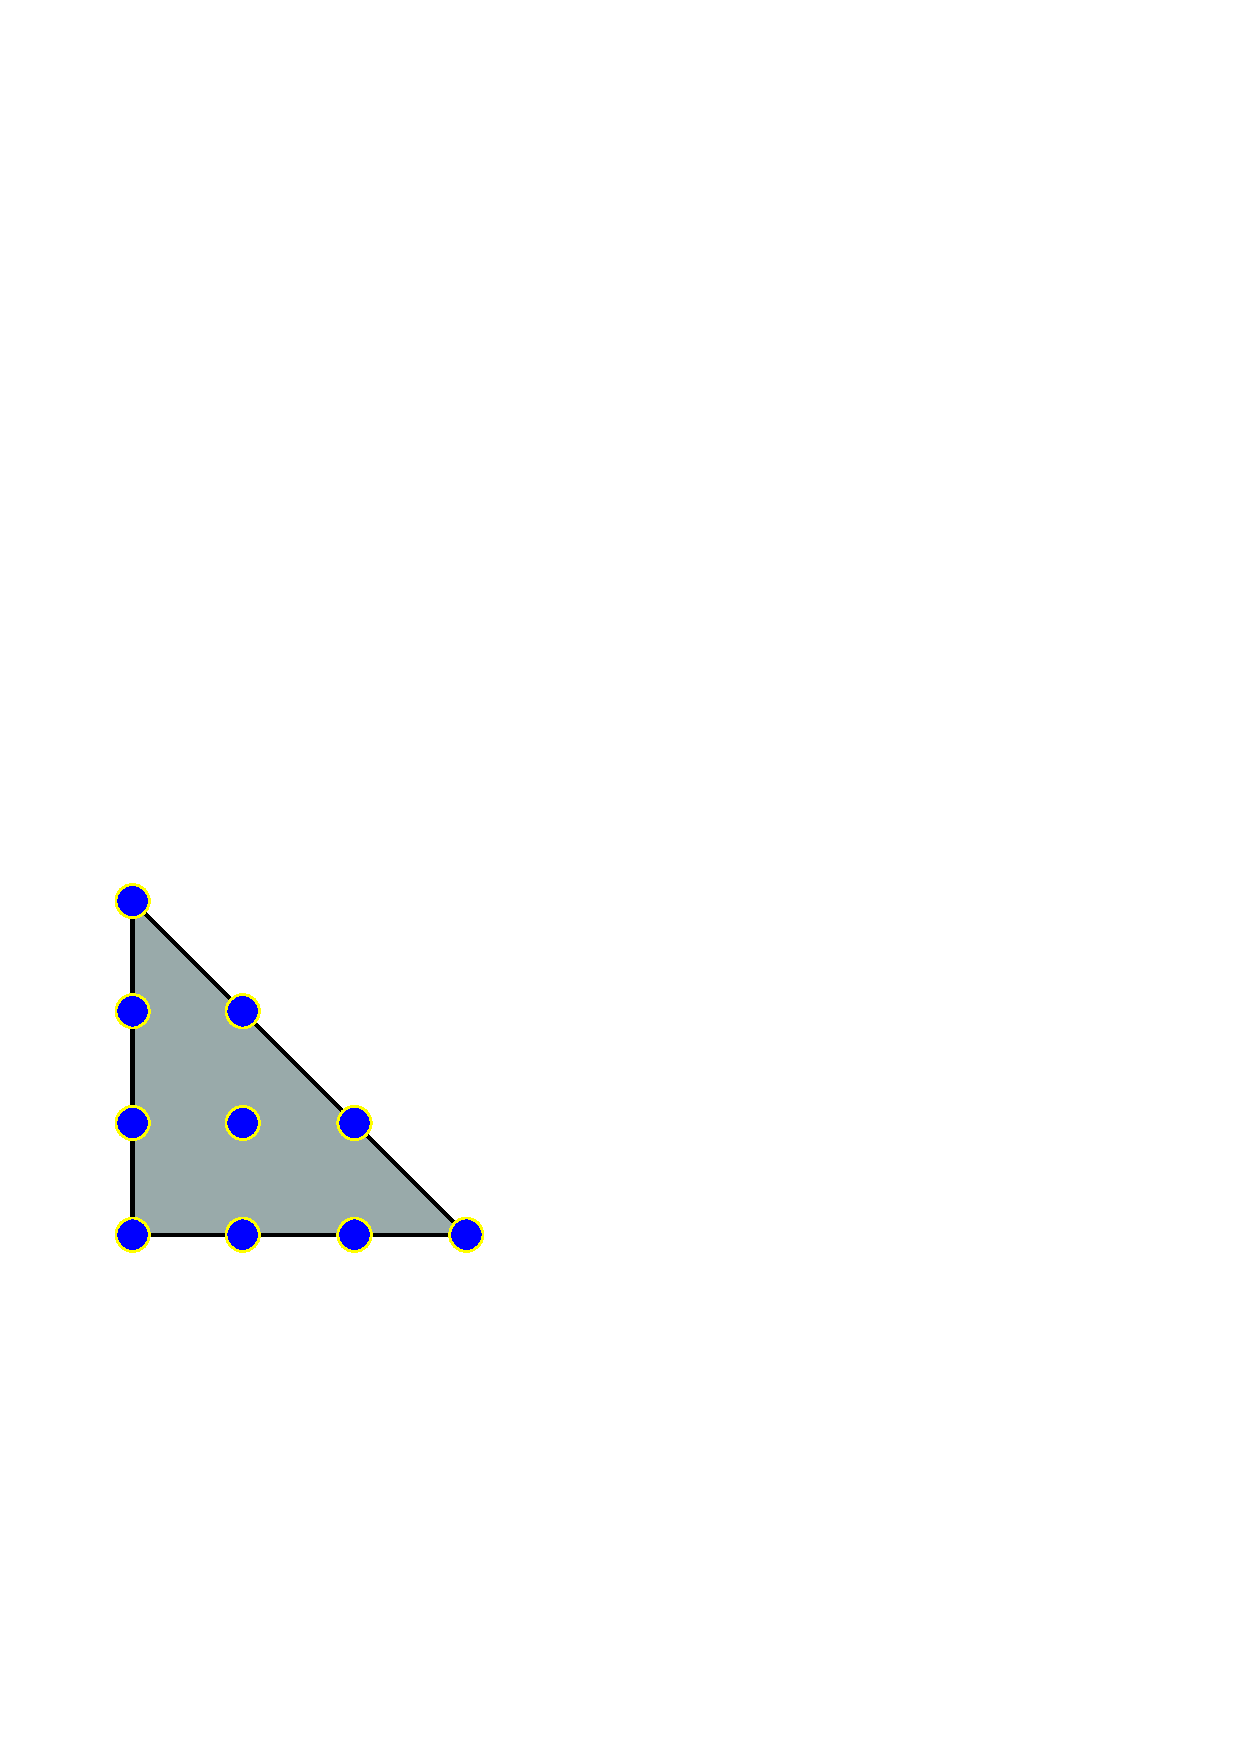
\includegraphics[width=.3\textwidth]{figures/part_4/P3FE.pdf}~~~~~~~~ 
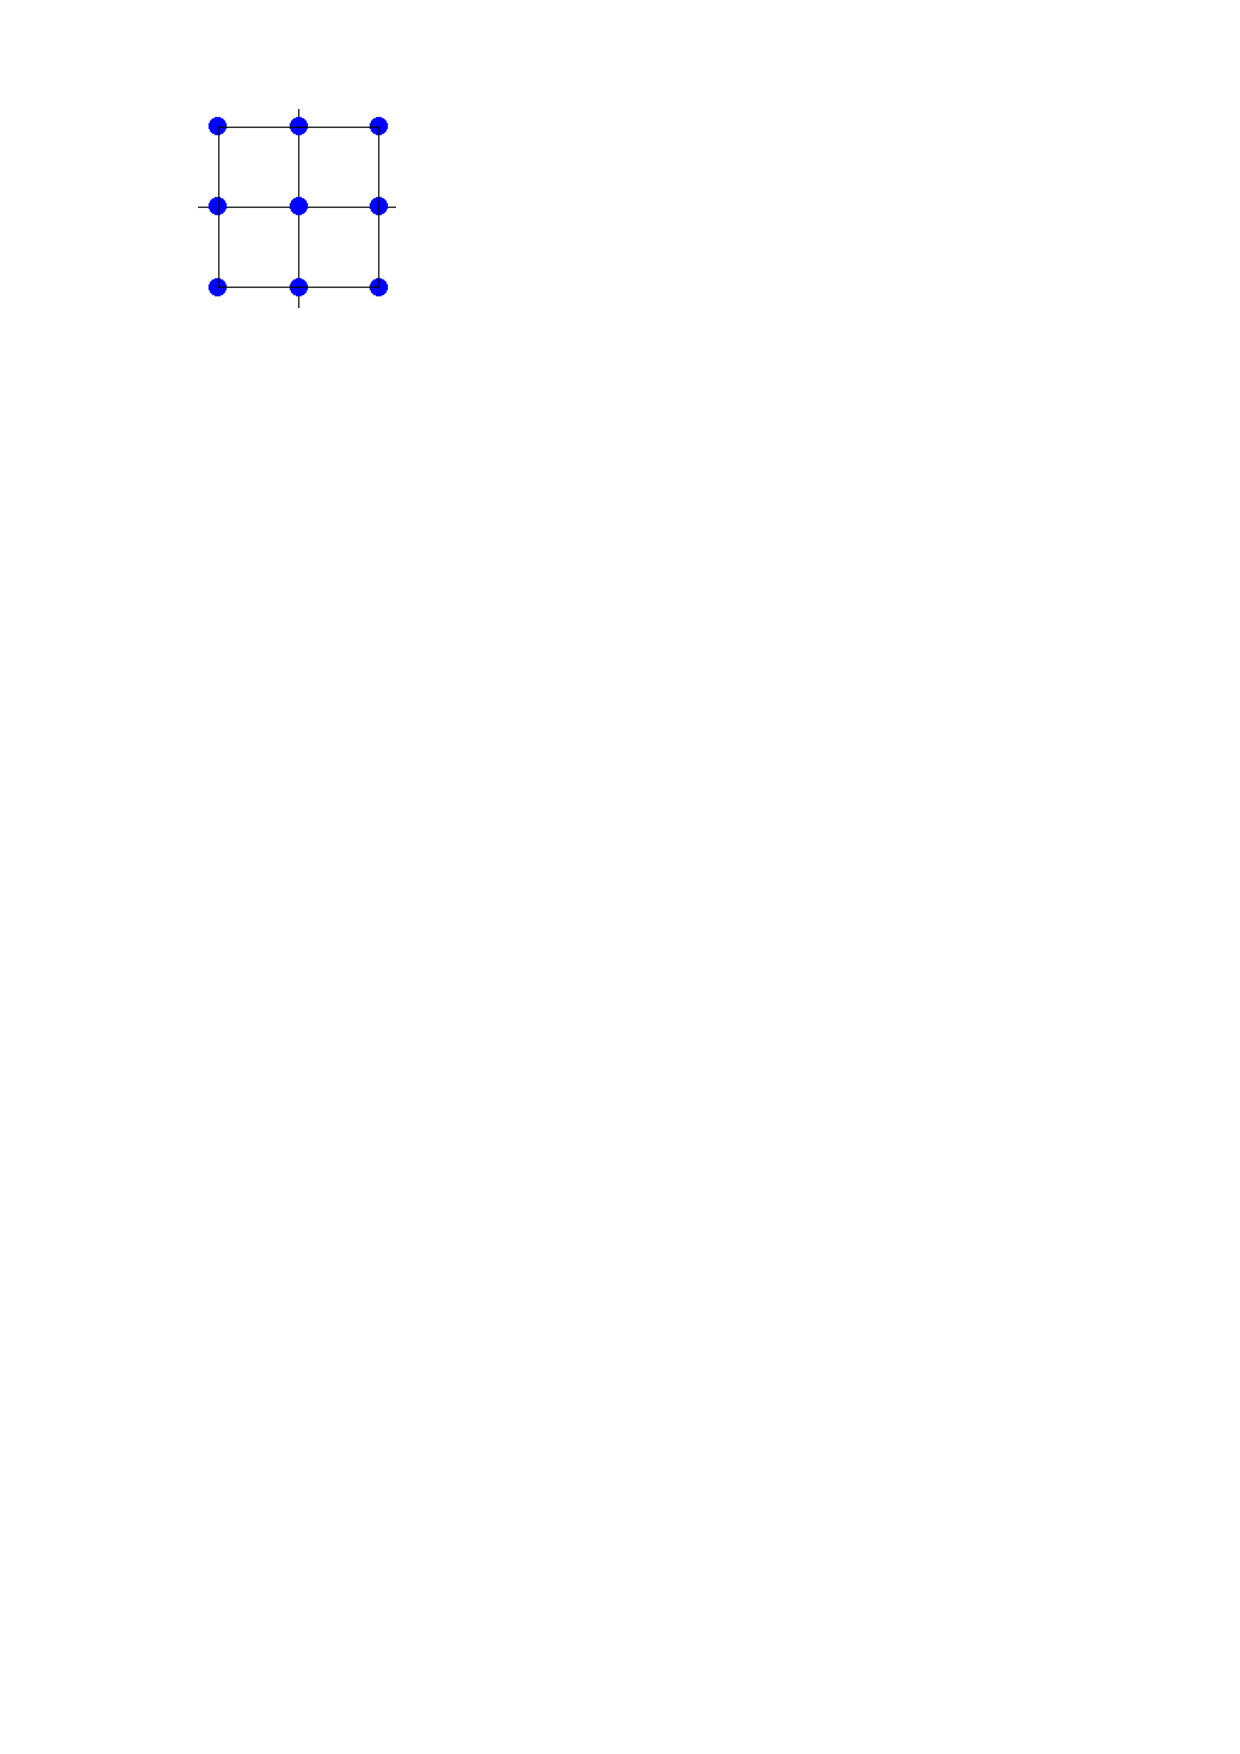
\includegraphics[width=.3\textwidth]{figures/part_4/Q2FE.pdf}}
\caption{\label{fig:FE} (Left) $\mathbb{P}_3$ Finite Element, (Right) $\mathbb{Q}_2$ Finite Element}
\end{figure}

\paragraph{Hypercube based $ \mathbb{Q}_k$ Finite Element.}
Let $K$ be the hypercube of dimension $n$ $K=\prod_{1\leq i \leq n} [a_i,b_i]$.
Let $P=\mathbb{Q}_k$ be the vector space of polynomials of degree $k$ in each direction:
$$ \mathbb{Q}_k=\{\mathrm{Span}(x_1^{\alpha_1} \dots x_n^{\alpha_n}), ~~~~ (\alpha_1,\dots,\alpha_n)\in \mathbb{N}^n, ~~~ 0\leq \alpha_1,\dots, \alpha_n \leq k   \}.$$
The degrees of freedom for this element is obtained by choosing $k+1$ distinct points $a_i=x_{i,0}< \dots < x_{i,k}=b_i$ in each direction.   The corresponding basis functions are the products in all directions of all the 1D Lagrange basis functions.
The Lagrange basis for $ \mathbb{Q}_k$ is $(l_{k,i_1}(x_1) \dots l_{k,i_n}(x_n))_{0\leq i_1,\dots,i_n \leq k}$, where the $l_{k,i_j}(x_j)$ denote the 1D Lagrange basis functions at the interpolation points $x_{j,0}, \dots, x_{j,k}$.
The dimension of $ \mathbb{Q}_k$ in $n$ dimensions is $(k+1)^n$, which is also the number of the basis functions.
An example with $k=2$ in 2D is given in Figure \ref{fig:FE}. Here the dimension of $ \mathbb{Q}_2$ is nine and the
nine basis functions are $l_{k,i}(x)l_{k,j}(y)$, $0\leq i,j\leq 2$. 


\subsection{$C^1$ Hermite Finite Elements}

Such elements are $H^2$ conforming and are needed when second order derivatives appear in the variational formulation. 

\paragraph{1D Hermite $ \mathbb{P}_{2k+1}$ Finite Element.} Hermite interpolation on an interval $[a,b]$ consists in finding a polynomial $p$ of degree $2k+1$ for $k \geq 1$, such that $p^{l}(a)$ and $p^l(b)$ are given for $0\leq l\leq k$. This will enforce $C^l$ continuity if all the interface degrees of freedom are shared.
To get $C^1$ continuity $k=1$ is enough:

\textit{Example $\mathbb{P}_3$ Hermite element in 1D.} This is the simplest possible Hermite Finite Element. 
Let $a,b\in \mathbb{R}$, $a<b$. Let $K=[a,b]$, 
$P= \mathbb{P}_3$ the linear space of cubic polynomials on $[a,b]$, $\Sigma=\{\sigma_1,
\sigma_2,\sigma_3, \sigma_4\}$, with
$$
\begin{array}{rcl}
\sigma_1:P&\rightarrow & \mathbb{R},\\
p&\mapsto &p(a),
\end{array}\qquad
\begin{array}{rcl}
\sigma_2:P&\rightarrow & \mathbb{R},\\
p&\mapsto &p(b),
\end{array}\qquad
\begin{array}{rcl}
\sigma_3:P&\rightarrow & \mathbb{R},\\
p&\mapsto &p'(a),
\end{array}
\begin{array}{rcl}
\sigma_4:P&\rightarrow & \mathbb{R},\\
p&\mapsto &p'(b).
\end{array}
$$

$C^1$ Finite Elements  are much more involved in higher dimensions at least for triangles and higher dimensional simplices than $C^0$ finite elements.  Tensor product constructions can be obtained from 1D Hermite Finite Elements, however they often have the constraint that the mapping also needs to be $C^1$, which is not the case for general affine mappings as are standardly used for $C^0$ Lagrange Finite Elements. Let us introduce the simplex examples on simplest triangle based and quad based $C^1$ finite elements.

\paragraph{Triangle $\mathbb{P}_3$ Hermite element.}

$K$ is a non degenerate triangle of vertices $ (\mathbf{a}_1, \mathbf{a}_2, \mathbf{a}_3)$, $P= \mathbf{P}_3$.
So $\dim P= 10$ and so ten degrees of freedom are needed. To enforce $C^1$ continuity, the value and the two components  of the gradient need to be fixed on each of the three vertices. This amounts to nine degrees of freedom, the tenth can be taken to be the value at the barycenter of the triangle.   This is represented on the left of Figure \ref{fig:C1FE}.

\paragraph{The Bogner-Fox-Schmitt rectangle $\mathbb{Q}_3$ Finite element.}
Taking the tensor product of two 1D $ \mathbf{P}_3$ Hermite Finite element. One obtains the Bogner-Fox-Schmitt element, which in addition to the point and two derivative values at each of the four vertices has also the cross derivative $\frac{\partial^2 p}{\partial x\partial y}$ as a degree of freedom. The corresponding basis consists of the products of all possible 1D cubic Hermite basis functions. Its dimension is $4\times 4=16.$
This is represented on the right of Figure \ref{fig:C1FE}.


\begin{figure}[ht]
\centerline{
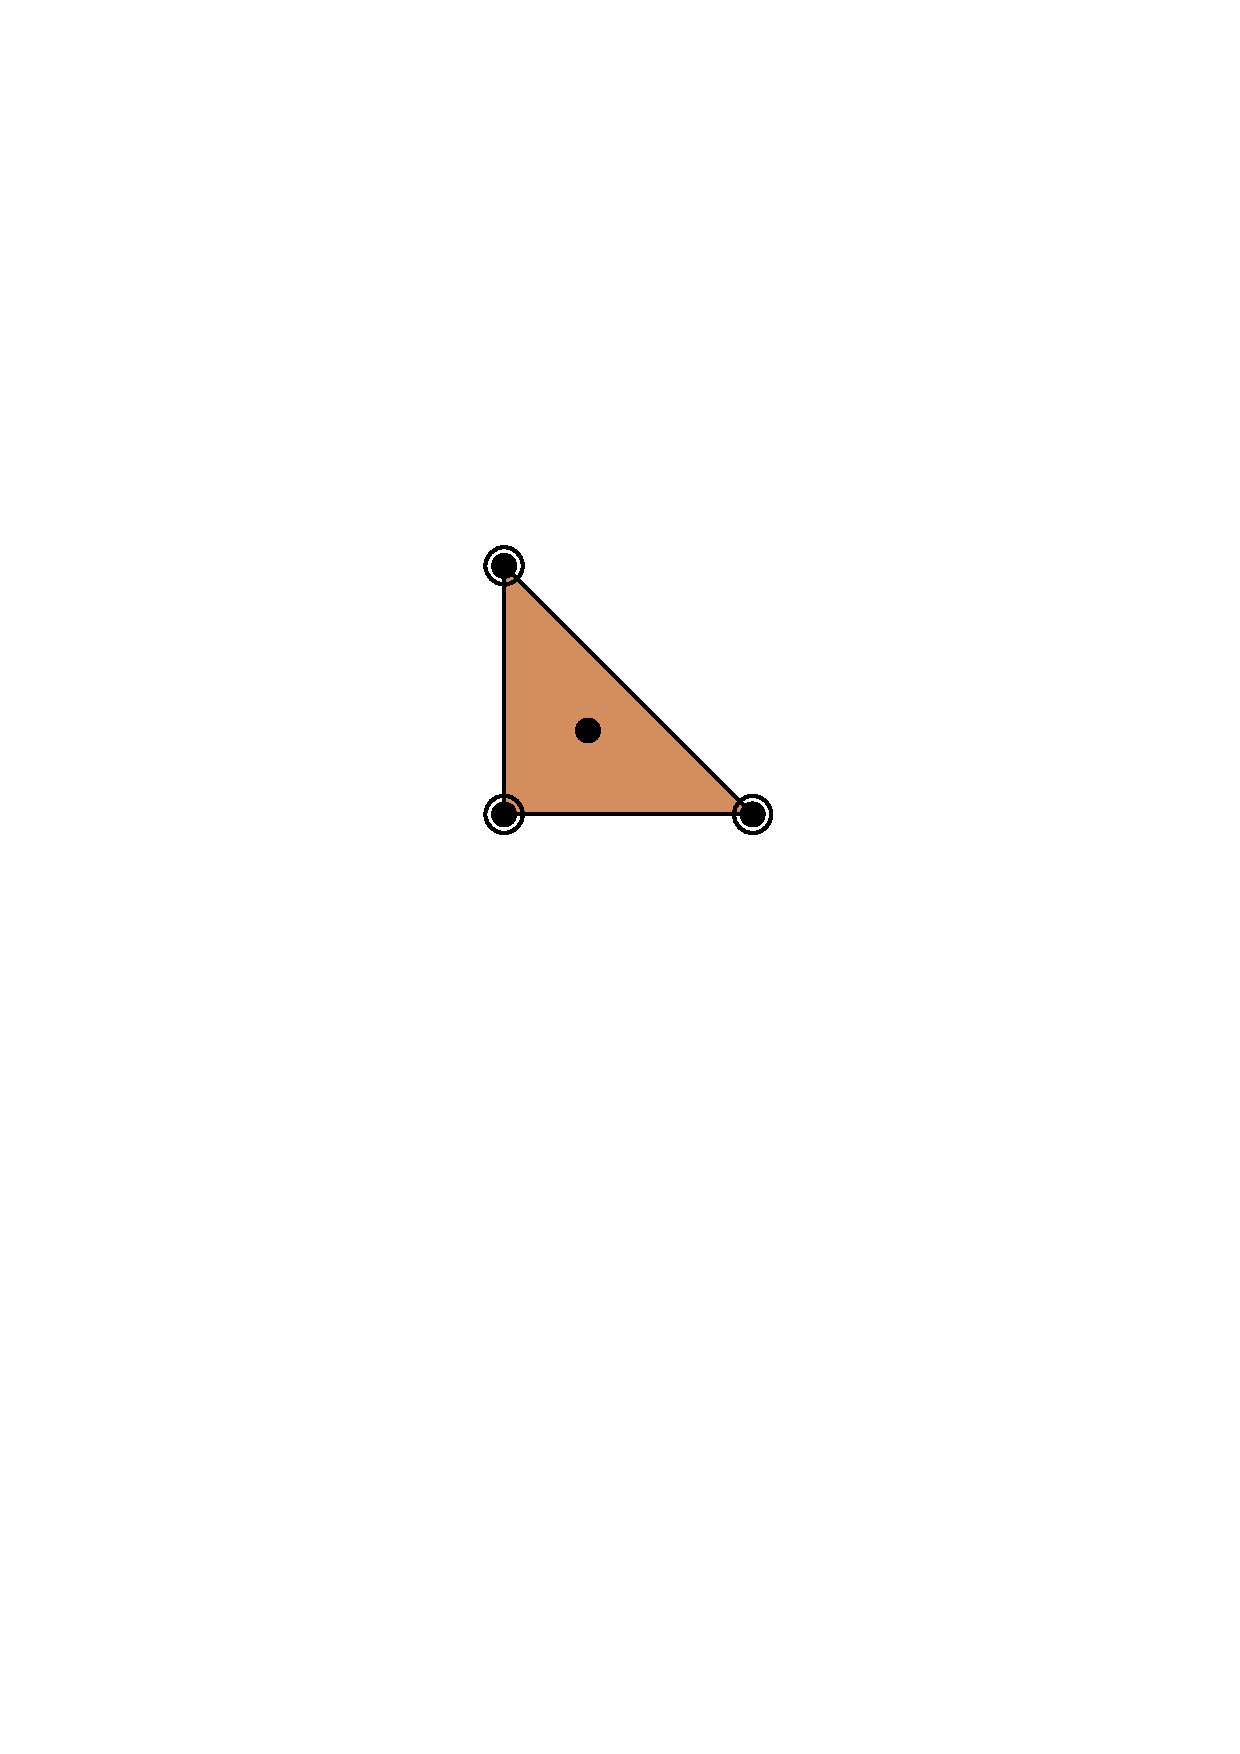
\includegraphics[width=.25\textwidth]{figures/part_4/HermiteTriangle.pdf}~~~~~~~~ 
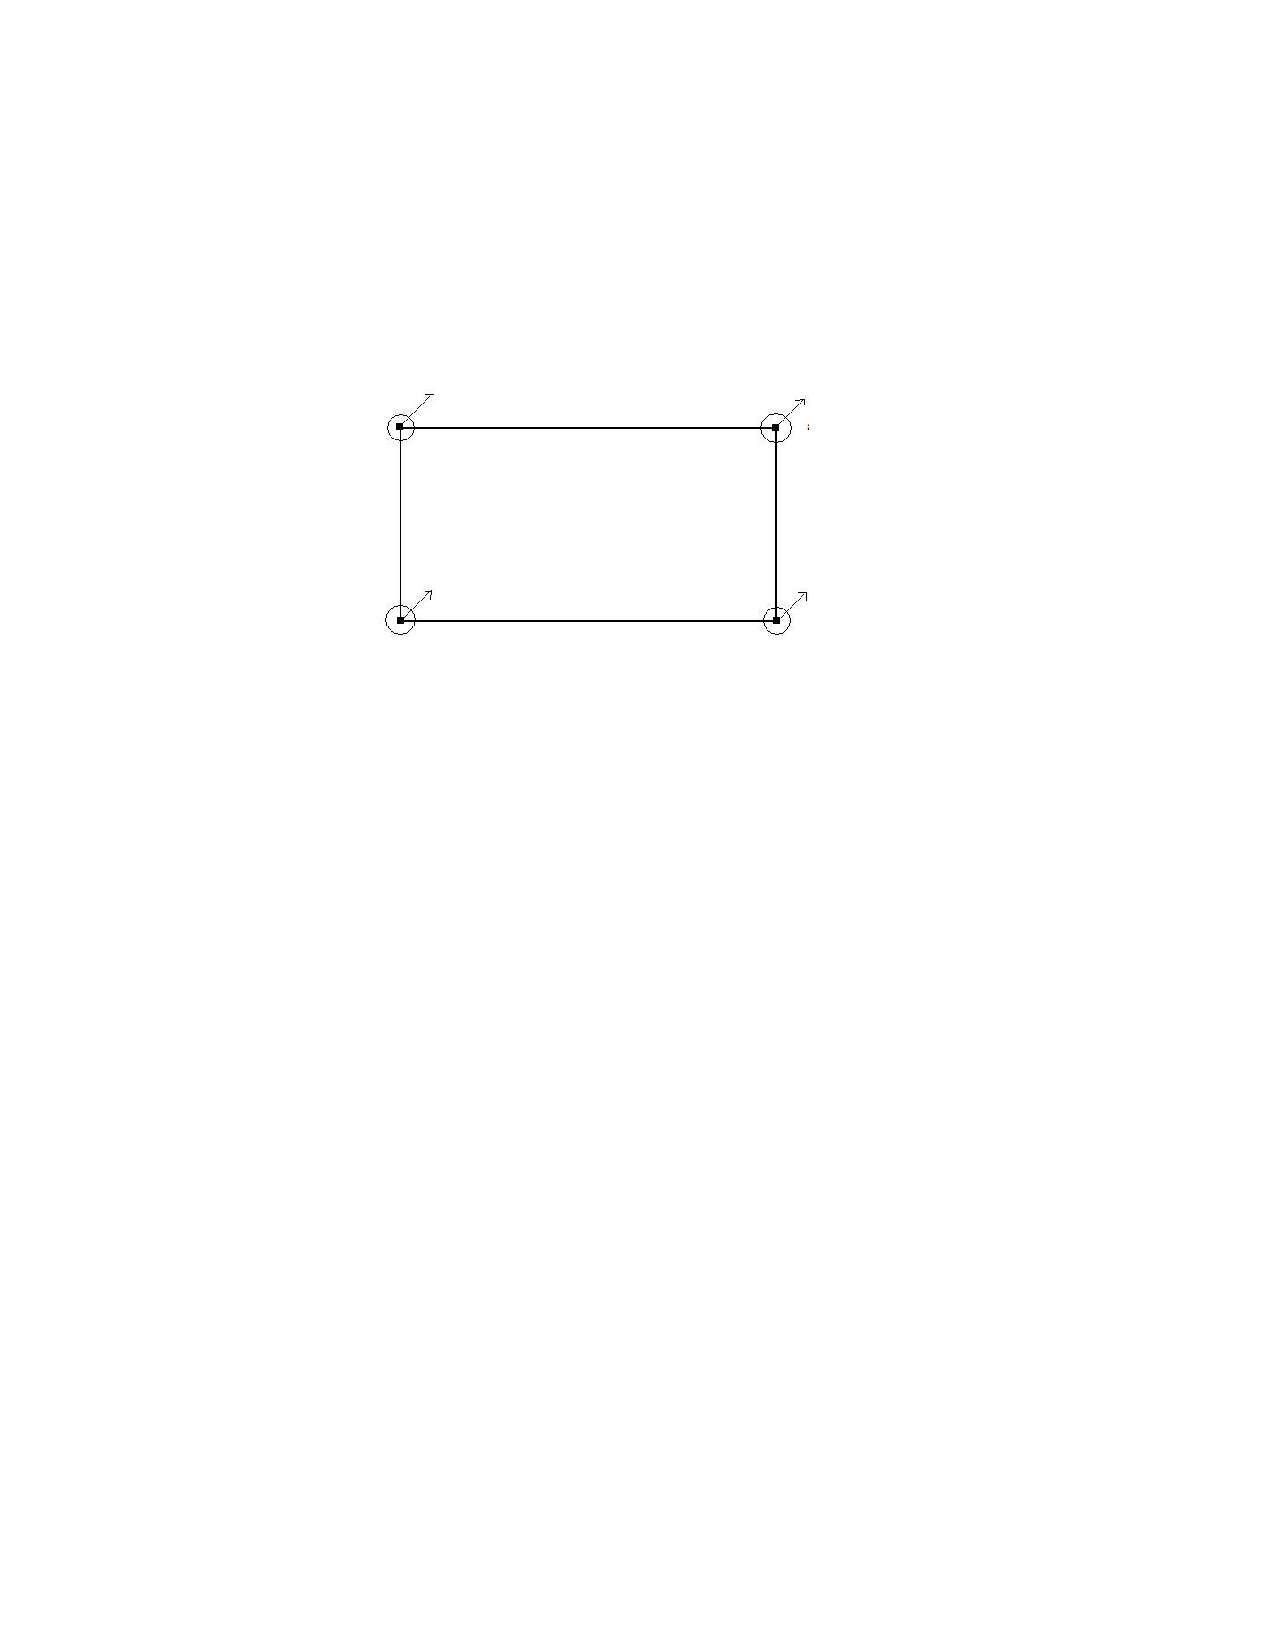
\includegraphics[width=.4\textwidth]{figures/part_4/BognerFoxSchmitt.pdf}}
\caption{\label{fig:C1FE} $C^1$ Finite Elements: (Left) $\mathbb{P}_3$ Hermite Finite Element, (Right) Bogner-Fox-Schmitt Finite Element}
\end{figure}


\subsubsection{Discontinuous finite elements}


Functions that are only in $L^2$ can be defined piecewise on each cell without any continuity requirements. 
Then there is no restriction on the degrees of freedom. 

Classical discontinuous Finite Elements are  \emph{nodal} Lagrange elements based on Gauss 
points as the quadrature points. Even though their approximation order is lower for the same number of points it is sometimes convenient to place the degrees of freedom at Gauss-Lobatto points, where one point on each side is on the edge. This makes easier the computation of edge integrals. However in this case, as the Finite Element is discontinuous, degrees of freedom on the interface are not shared by neighbouring elements. 

Another class of classical discontinuous Finite Elements are \emph{modal} elements where the basis functions are generally taken to be the orthonormal Legendre polynomials $(L_i)_{0\leq i \leq k}$, which have the advantage of  yielding the identity as a mass matrix. The corresponding degrees of freedom are
$\sigma_i(p) = \int p(x) L_i(x) \dd x.$ 
Such constructions, where each element of the basis has a deferent degree, are called hierarchical finite elements and facilitate what is called the $p$ refinement consisting in obtaining a more accurate approximation by taking a higher order polynomial rather that refining the grid. Indeed in this case when refining only one basis function needs to be added to the existing one rather than replacing all the basis functions as would be necessary for the previously seem Finite Elements where all basis functions have the same degree. 


\subsection{ $H(\textrm{div}, \Omega)$ conforming Finite Elements}

The $H(\textrm{div}, \Omega)$ space consists of vector fields. Each element as $n$ components in  $n$ dimensions. Moreover, as we have seen before $H(\textrm{div}, \Omega)$ vector fields have a continuous normal component and a discontinuous tangential component. Let us explain how such elements can be constructed in two dimensions. This can be generalised to higher dimensions. 

\paragraph{Tensor product construction.} Due to the given continuity requirements a $H(\textrm{div}, \Omega)$ conforming Finite Element can be constructed, by defining separately an approximation of the tangential component and of the normal component. 
In this case $K=[-1,1]\times [-1,1]$, 
$$ P = \{ \mathbf{p}=(p_x,p_y)^\top \,|\, p_x\in \mathbb{Q}_{k-1,k}, p_y\in \mathbb{Q}_{k,k-1}\},$$
where 
$$ \mathbb{Q}_{m,n}= \mathrm{Span} ( x^\alpha y^\beta,  ~ 0\leq \alpha\leq m, 0\leq \beta\leq n).$$
For $p_x$ the degrees of freedom are the Gauss points in $x$ and the Gauss-Lobatto points in $y$, such that $p_x$ is discontinuous in $x$ and continuous in $y$. It is the other way for $p_y$.
This enables arbitrarily high order   $H(\textrm{div}, \Omega)$ conforming elements.

\paragraph{The Raviart-Thomas (RT) Finite Element.}

$K$ is a non degenerate triangle of vertices $ (\mathbf{a}_1, \mathbf{a}_2, \mathbf{a}_3)$. For the element of order $k+1$, $k\geq 0$, denoting by $\bar{ \mathbb{P}}_k$ the space of homogeneous polynomials of degree $k$ (\textit{i.e.} all the monomials are exactly of degree $k$)
$$P = RT_k = (\mathbb{P}_k)^2 + 
\begin{pmatrix} x\\ y \end{pmatrix} \bar{ \mathbb{P}}_k.
$$
In two dimensions $\dim \mathbb{P}_k = (k+1)(k+2)/2$ and $\dim \bar{\mathbb{P}}_k = k+1$, so that
$\dim RT_k = (k+1)(k+3)$. This yields in particular $\dim RT_0= 3$, $\dim RT_1= 8$, $\dim RT_2= 15$.
The degrees of freedom are constructed starting from the edges in order to enforce the continuity requirements. This is our first example of moment based degrees of freedom, defined by 1D moments along the edges to enforce continuity and then 2D moments in the triangle to complete the missing degrees of freedom. 
$$\Sigma=\left\{ \mathbf{p}\mapsto\int_{e_i} \mathbf{p}\cdot \un s^l\dd s, 0\leq l\leq k,~~~  
\mathbf{p}\mapsto\int_K \mathbf{p}(x_1,x_2) \cdot x_i^l \dd x_i, ~~  0\leq l\leq k-1, ~i=1,2\right\}.  $$
We count here $k+1$ degrees of freedom for each of the three edges, and  $2k$ inner degrees of freedom,
which are in total $3(k+1)+ 2k(k+1)/2 = (k+1)(k+3)$ which is precisely the dimension of $RT_k$. To prove the unisolvence it is thus enough to prove that a polynomial which vanishes on all degrees of freedom is necessarily zero. Note that because the monomials in our degrees of freedom are a basis of the polynomial spaces
$ \mathbb{P}_k(e_i), ~i=1,2,3$ and  $ \mathbb{P}_{k-1}(K)$ respectively this is given by the following lemma:
\begin{lemma} Let $k\geq 0$, and $ \mathbf{p}\in RT_k(K)$ then
\begin{align}
\int_{e_i} \mathbf{p}\cdot \un \,r \dd s &=0, \quad \forall r\in \mathbb{P}_k(e_i), \label{eq:RTe}\\
\int_K \mathbf{p}  \cdot \mathbf{q} \dd \mathbf{x} &=0 \quad\forall \mathbf{q} \in (\mathbb{P}_{k-1})^2
\label{eq:RTf}
\end{align}
implies that $ \mathbf{p}=0$.
\end{lemma}

\begin{remark}
Note that instead of the monomials one can use \eqref{eq:RTe} and  \eqref{eq:RTf} applied to arbitrary bases of 
$\mathbb{P}_k(e_i)$ and $(\mathbb{P}_{k-1})^2$ respectively.
\end{remark}


\begin{proof}
Let $ \mathbf{p} \in RT_k$. Then $ \mathbf{p} = \mathbf{q} + \begin{pmatrix} x\\ y \end{pmatrix} \psi$
with $\mathbf{q}\in (\mathbb{P}_k)^2$ and $\psi\in \bar{ \mathbb{P}}_k$.
Let us first observe that on any of the three edges $e_i$ we have
  $ \mathbf{p}\cdot \un\in \mathbb{P}_k(e_i)$, this is obvioulsy the case for
$ \mathbf{p}\cdot \un$. On the other hand if $(x(s),y(s))$ defines a parametrisation of $e_i$, then
by definition of the normal $n_x (x(s)-x(s_0)) + n_y (y(s)-y(s_0)) = 0$ so that
$n_x x(s) + n_y y(s)$ is constant on $e_i$. It follows that on the edge $e_i$
$$ \un\begin{pmatrix} x\\ y \end{pmatrix} \psi= (n_x x + n_yy)\psi.$$
Then as $(n_x x + n_yy)$ is a constant, $n_x x + n_yy)\psi$ is a polynomial of degree $k$ like $\psi$.

Now  computing the divergence of  $\mathbf{p}$ we find
$$\nabla\cdot \mathbf{p} = \nabla\cdot \mathbf{q} + 2\psi + \begin{pmatrix} x\\ y \end{pmatrix} \cdot \nabla\psi
= \nabla\cdot \mathbf{q}  + (k+2)\psi. $$
Hence $ \nabla\cdot \mathbf{p}$ is a polynomial of degree $k$ orthogonal to all polynomials of degree k. Thus it is 0. Then because $\nabla\cdot \mathbf{q} \in \mathbb{P}_{k-1}$ it also follows that $\psi=0$ and hence
$\mathbf{p}\in (\mathbb{P}_k)^2$.


Let us take $\varphi\in \mathbb{P}_k$. Then $\nabla\varphi\in (\mathbb{P}_{k-1})^2$ and hence using
\eqref{eq:RTf} we get using a Green's formula
$$\int_K \mathbf{p}  \cdot \nabla\varphi \dd \mathbf{x} =0 = \int_{\partial K}  \mathbf{p}\cdot \un\varphi \, \dd s + \int_K \nabla\cdot \mathbf{p} \, \varphi \dd \mathbf{x}.$$
As the boundary term vanishes due to \eqref{eq:RTe}, it follows that $\int_K \nabla\cdot \mathbf{p} \, \varphi \dd \mathbf{x}=0$. This for all $\varphi\in \mathbb{P}_k$.


Now in order to conclude we assume that the reference triangle has one edge on $x=0$ and one edge on $y=0$ and is in the positive quarter plane.
The the condition $ \mathbf{p}\cdot \un=0$ yields that $p_x=0$ for $x=0$, hence $p_x= x\psi_1$ with
$\psi_1\in \mathbb{P}_{k-1}$ and $p_y=0$ for $y=0$, hence $p_y= y\psi_2$ with
$\psi_2\in \mathbb{P}_{k-1}$. Then taking $\mathbf{q}=(\psi_1,\psi_2)^\top$ in \eqref{eq:RTf}, we obtain
$$\int_K (x\psi_1^2 +y\psi_2^2) \dd \mathbf{x}=0$$
from which it follows as both terms are positive that they are both zero. So $ \mathbf{p}=0$ which was what we needed to prove.
\end{proof}

\begin{remark}
Obviously, the procedure used here to construct the Finite Element, by first setting the boundary degrees of freedom to ensure the required continuity and then complete with the needed inner degrees of freedom can also be applied to quads.
\end{remark}




\paragraph{The Brezzi-Douglas-Marini (BDM) Finite Element.}
$K$ is a non degenerate triangle of vertices $ (\mathbf{a}_1, \mathbf{a}_2, \mathbf{a}_3)$. 
Here $P$ is the full polynomial space in each direction $P = BDM_k = (\mathbb{P}_k)^2 $. As continuity of the normal component is needed on each of the three faces, these requires at least three degrees of freedom. So and $ H(\textrm{div}, \Omega)$ conforming $BDM_k$ element can only be constructed for $k\geq 1$ as $\dim BDM_0=2$. In order to define the degrees of freedom, we need the following space
$$N_k = (\mathbb{P}_k)^2 + \begin{pmatrix} y\\ -x \end{pmatrix} \bar{ \mathbb{P}}_k, $$
This space has obviously the same dimension as the corresponding $RT_k$: $\dim N_k=\dim RT_k=(k+1)(k+3)$.
We can now define the degrees of freedom for the $BDM_k$ element:
introducing $(\psi_j)_0\leq j\leq k$ a basis of $ \mathbb{P}_k$ on each edge (this could be the monomials $s^j$ as we used for Raviart-Thomas or any other basis), and $(\boldsymbol{\varphi}_j)_{0\leq (k-1)(k+1)}$ a basis of $N_{k-2}$
\begin{multline*}
\Sigma=\left\{ \mathbf{p}\mapsto\int_{e_i} \mathbf{p}\cdot \un \psi_j\dd s, 0\leq j\leq k,~i=1,2,3, \right.\\ \left.
\mathbf{p}\mapsto\int_K \mathbf{p} \cdot \boldsymbol{\varphi}_j \dd \mathbf{x} , ~~ 0\leq j\leq  (k-1)(k+1) \right\}.
\end{multline*}
We first notice, that the number of degrees of freedom is $3(k+1) + (k-1)(k+1)=(k+1)(k+2)=\dim P$. So that proving that  $ \mathbf{p}\in P$ must vanish if all these degrees of freedom are zero is enough to prove unisolvence. Similarly as for the Raviart-Thomas element this follows from the following:
\begin{lemma} Let $k\geq 1$, and $ \mathbf{p}\in \mathbb{P}_k(K)^2$ then
\begin{align}
\int_{e_i} \mathbf{p}\cdot \un \,\psi \dd s &=0, \quad \forall \psi\in \mathbb{P}_k(e_i), \label{eq:BDMe}\\
\int_K \mathbf{p}  \cdot \mathbf{q}\dd \mathbf{x} &=0 \quad\forall \mathbf{q}\in N_{k-2}
\label{eq:BDMf}
\end{align}
implies that $ \mathbf{p}=0$.
\end{lemma}

\begin{proof}
Let $ \mathbf{p}\in \mathbb{P}_k(K)^2$ verifying \eqref{eq:BDMe} and \eqref{eq:BDMf}. 
For any $\varphi\in \mathbb{P}_{k-1}$, we have that $\nabla\varphi\in (\mathbb{P}_{k-2})^2\subset N_{k-2}$, hence from
\eqref{eq:BDMf} it follows that 
$$\int_K \mathbf{p}  \cdot \nabla\varphi \dd \mathbf{x} =0 = -\int_K \nabla\cdot \mathbf{p}\, \varphi \dd x
+\int_{\partial K} \mathbf{p}\cdot \un \, \varphi\dd s. $$

The last term is zero because of \eqref{eq:BDMe}. Then $\nabla\cdot \mathbf{p}$ is a polynomial of degree $k-1$ orthogonal to all polynomials of degree $k-1$. Hence it is zero.
Thus $ \mathbf{p}= (\partial_y \psi, -\partial_x \psi)$ for a $\psi\in \mathbb{P}_{k+1}$. Moreover due
to  \eqref{eq:BDMe},  $ \mathbf{p}\cdot \un=0$ on each edge, this implies that the tangential derivative of $\psi$ on each edge, and so $\psi$ is constant on all the edges. As it is defined up to a constant, on can choose $\psi$ such that it vanishes on the three edges. Then introducing the barycentric coordinates $\lambda_1, \lambda_2, \lambda_3$ of the triangle, it follows that each $\lambda_i$ divides $\psi$, so that
$\psi=\lambda_1\lambda_2\lambda_3 \tilde{\psi}$ with $\tilde{\psi}\in \mathbb{P}_{k-2}$.

Let us now take $ \mathbf{q} =   \begin{pmatrix} y\\ -x \end{pmatrix} \tilde{\psi} \in N_{k-2}$. Then from 
\eqref{eq:BDMf} it follows that
$$\int_K \mathbf{p}  \cdot \mathbf{q}\dd \mathbf{x} = \int_K \begin{pmatrix} \partial_y \psi \\ -\partial_x \psi \end{pmatrix}\cdot \begin{pmatrix} y\\ -x \end{pmatrix} \tilde{\psi}\dd \mathbf{x}=
\int_K k\lambda_1\lambda_2\lambda_3 \tilde{\psi}^2 \dd x=0$$
which implies that $ \tilde{\psi}=0$ and thus $ \mathbf{p}=0$, which is the desired result.
\end{proof}

\begin{figure}[ht]
\centerline{
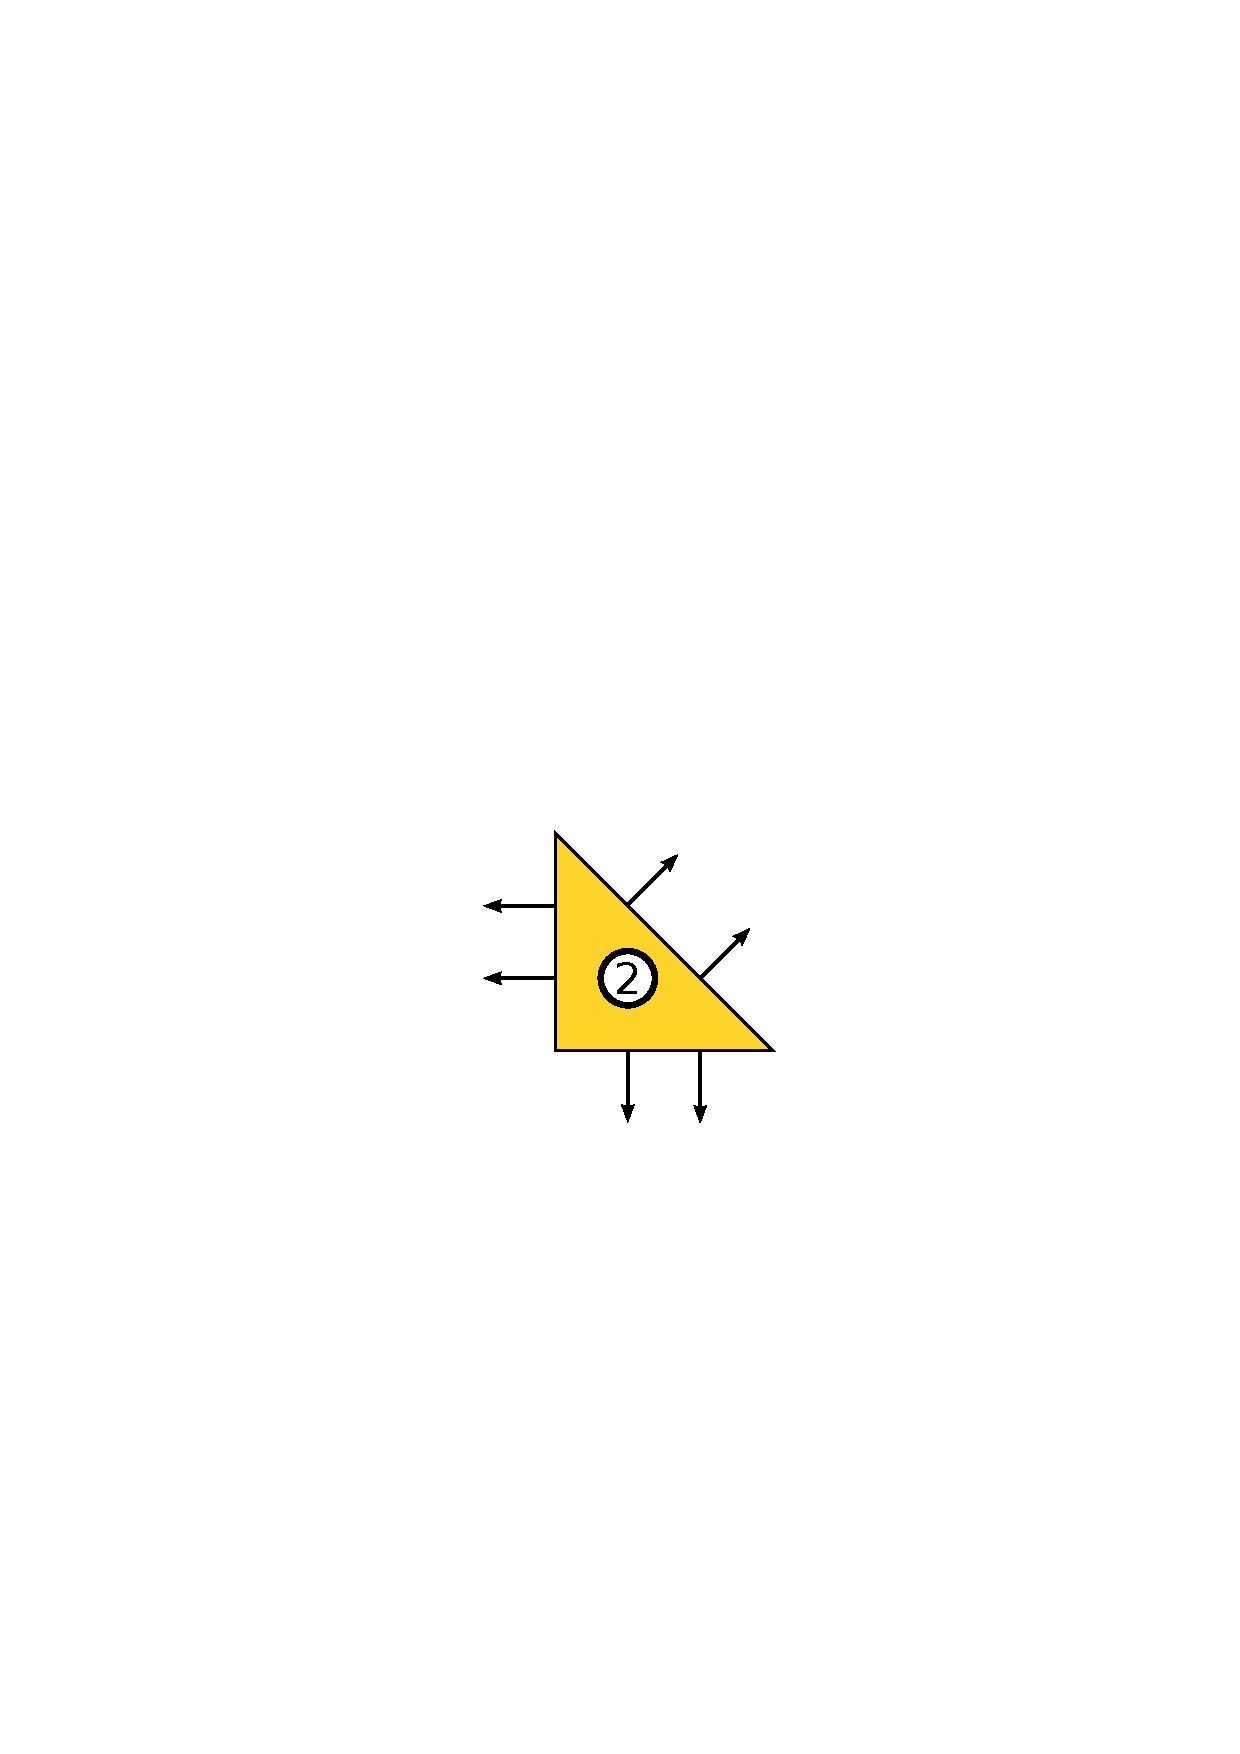
\includegraphics[width=.3\textwidth]{figures/part_4/RT1.pdf}~~~~~~~~ 
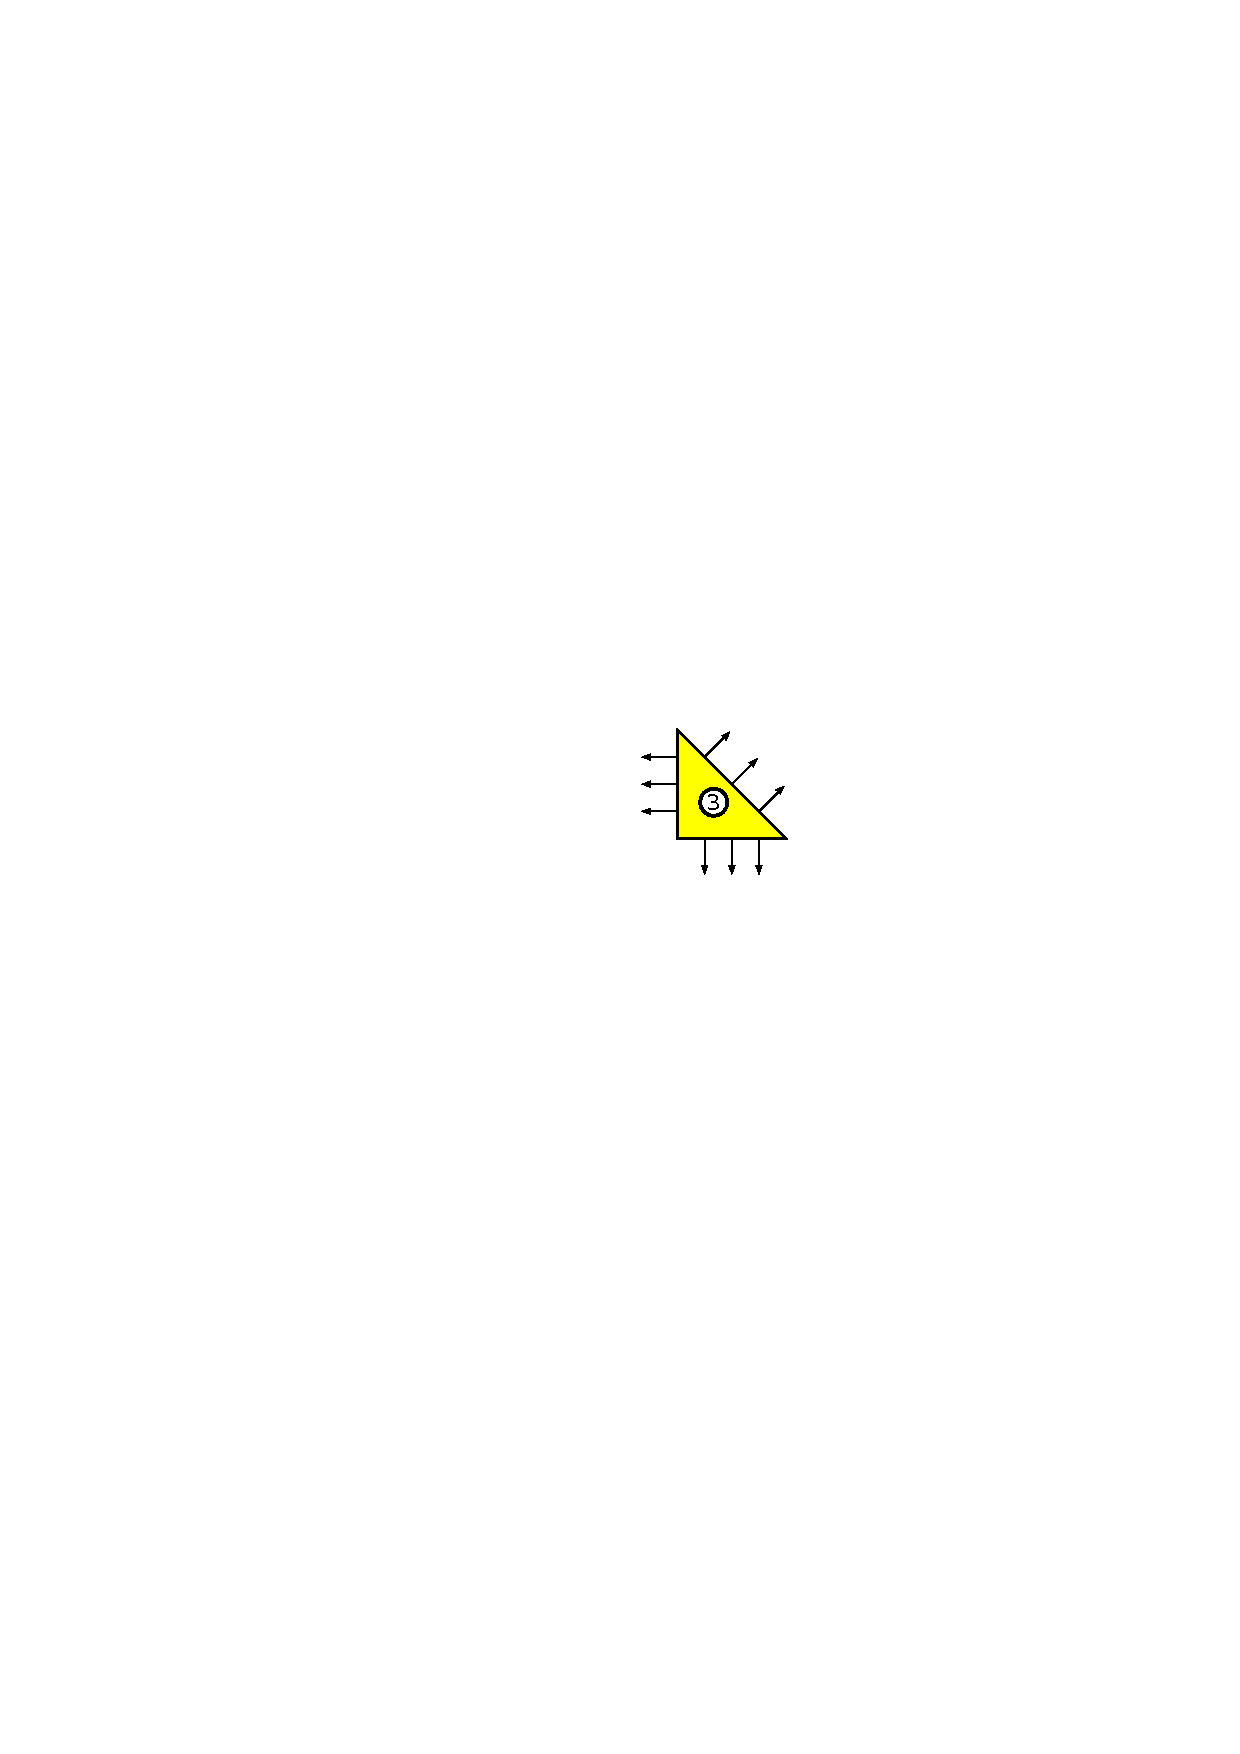
\includegraphics[width=.3\textwidth]{figures/part_4/BDM2.pdf}}
\caption{\label{fig:HdivFE} $H(div)$ Finite Elements: (Left) $RT_1$ Raviart-Thomas Element, (Right) $BDM_2$ Brezzi-Douglas-Marini Element}
\end{figure}

\begin{remark}
The extension to 3D is straightforward, the degrees of freedom stay the same, the triangles being replaced by tetrahedra and the edges being replaced by faces.
\end{remark}


\subsection{ $H(\textrm{curl}, \Omega)$ conforming Finite Elements}

Recall that for a 3D vector $\mathbf{u}=(u_1,u_2,u_3)^\top$, the curl is defined by the relation
$$ \nabla\times \mathbf{u} = \begin{pmatrix}
\partial_2 u_3 - \partial_3 u_2 \\ \partial_3 u_1 - \partial_1 u_3 \\ \partial_1 u_2 - \partial_2 u_1 
\end{pmatrix}.$$
In 2D, there is no dependency on the third coordinate and the curl degenerates into the vector curl of a scalar, for the first two components and the scalar curl of a vector for the last component:
$$ \nabla\times \mathbf{u} =
  \begin{pmatrix}
  \mathbf{curl}\, u_3 \\  \mathrm{curl}\, \underline{\mathbf{u}}
  \end{pmatrix}~~~~
  \mbox{ with }  
  \mathbf{curl}\, u_3 =  \begin{pmatrix}
\partial_2 u_3  \\  - \partial_1 u_3
\end{pmatrix}, ~~
\underline{\mathbf{u}} =  \begin{pmatrix}
u_1  \\  u_2
\end{pmatrix}, ~~
\mathrm{curl}\, \underline{\mathbf{u}} = \partial_1 u_2 - \partial_2 u_1.
$$

$ H(\textrm{curl}, \Omega)$ conforming elements have a continuous tangential component. They can thus be simply obtained in 2D by exchanging the two components of the vector in the tensor product case.

For triangles, the natural finite element space, built as the Raviart-Thomas element is the N\'ed\'elec Element defined by $K=( \mathbf{a}_1, \mathbf{a}_2, \mathbf{a}_3)$, a non degenerate triangle,
$$P=N_k = (\mathbb{P}_k)^2 + \begin{pmatrix} y\\ -x \end{pmatrix} \bar{ \mathbb{P}}_k, $$
and the degrees of freedom are obtained from the Raviart-Thomas degrees of freedom by replacing the normal  $\un=(\nu_1,\nu_2)^\top$ by the tangent $ \ut=(\nu_2,-\nu_1)$. 
Unisolvence is also easily adapted from the Raviart-Thomas case and is based on the following 
\begin{lemma} Let $k\geq 0$, and $ \mathbf{p}\in RT_k(K)$ then
\begin{align}
\int_{e_i} \mathbf{p}\cdot \ut \,r \dd s &=0, \quad \forall r\in \mathbb{P}_k(e_i), \label{eq:Ne}\\
\int_K \mathbf{p}  \cdot \mathbf{q} \dd \mathbf{x} &=0 \quad\forall \mathbf{q} \in (\mathbb{P}_{k-1})^2
\label{eq:Nf}
\end{align}
implies that $ \mathbf{p}=0$.
\end{lemma}


\begin{figure}[ht]
\centerline{
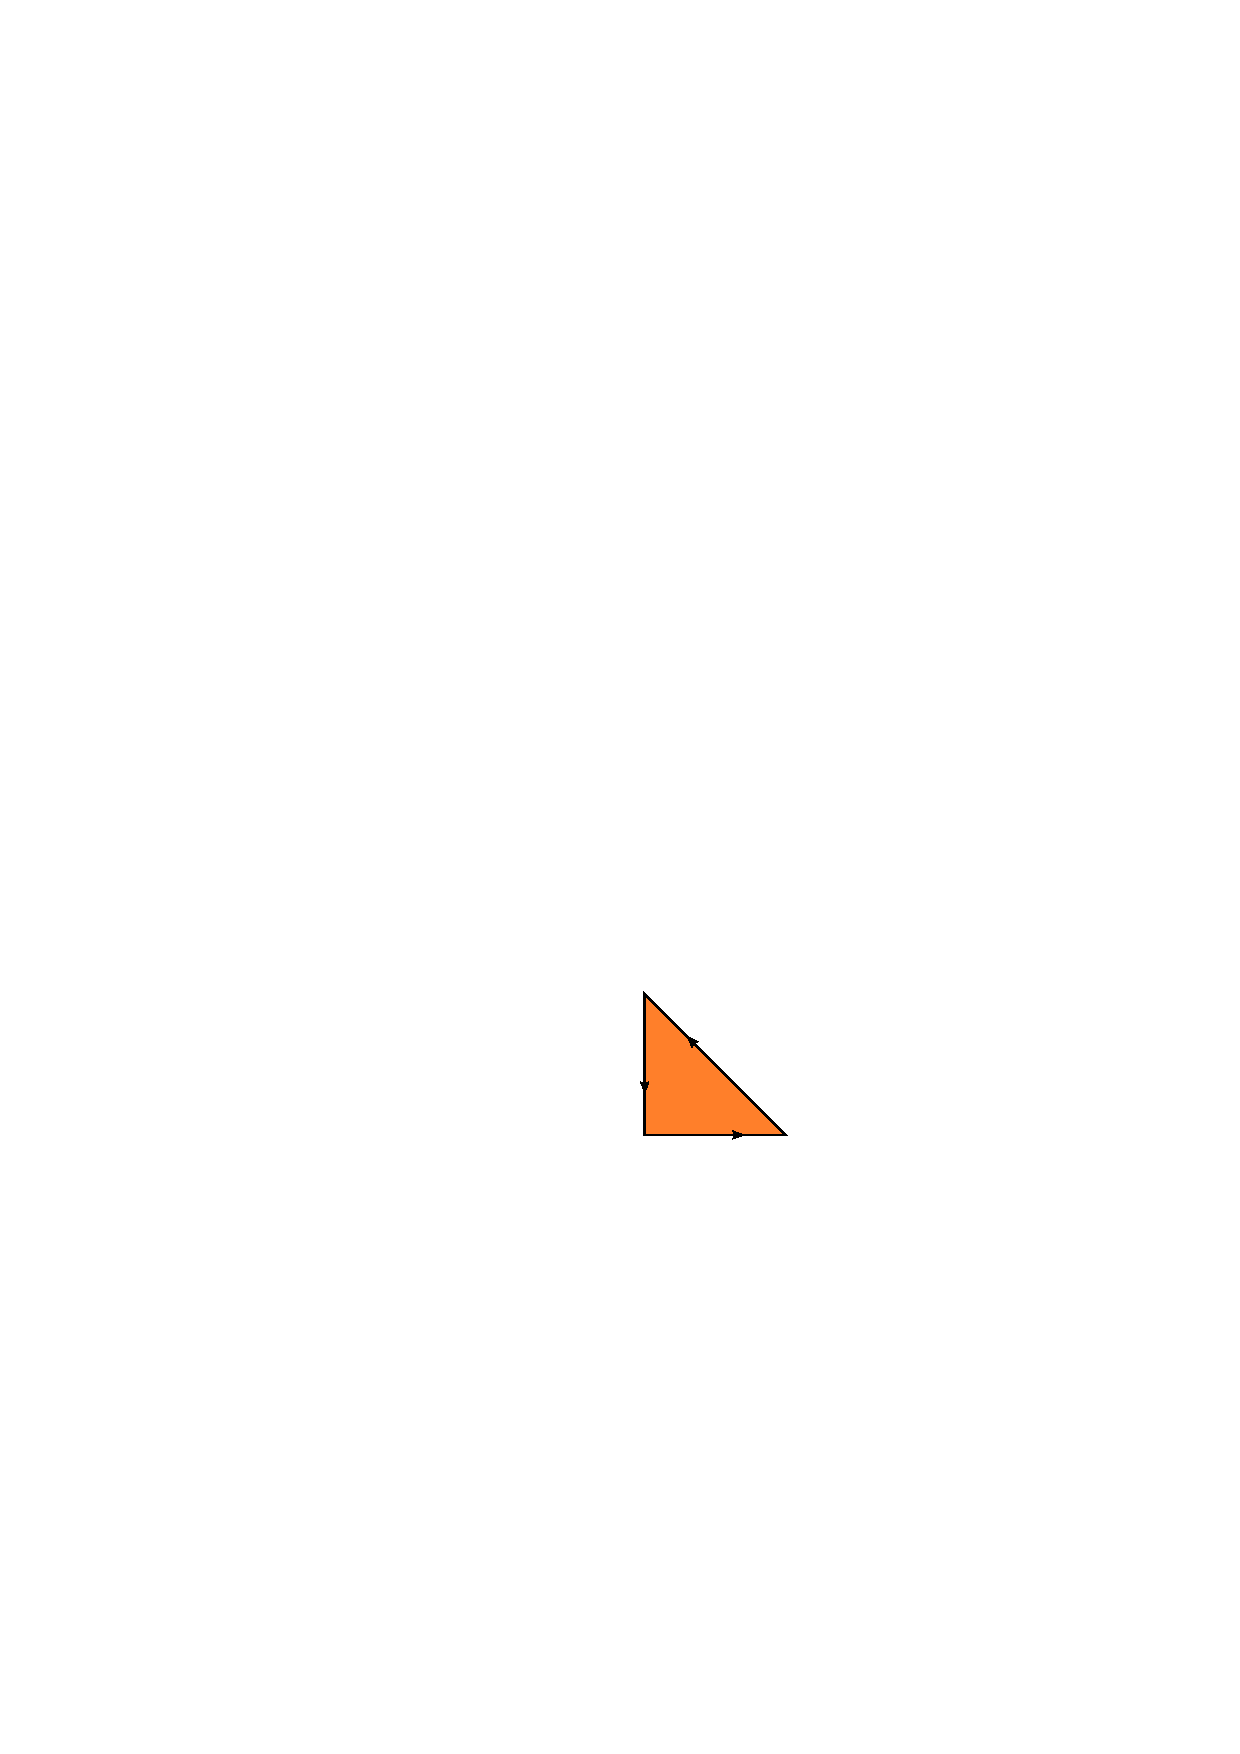
\includegraphics[width=.3\textwidth]{figures/part_4/Ned0.pdf}~~~~~~~~ 
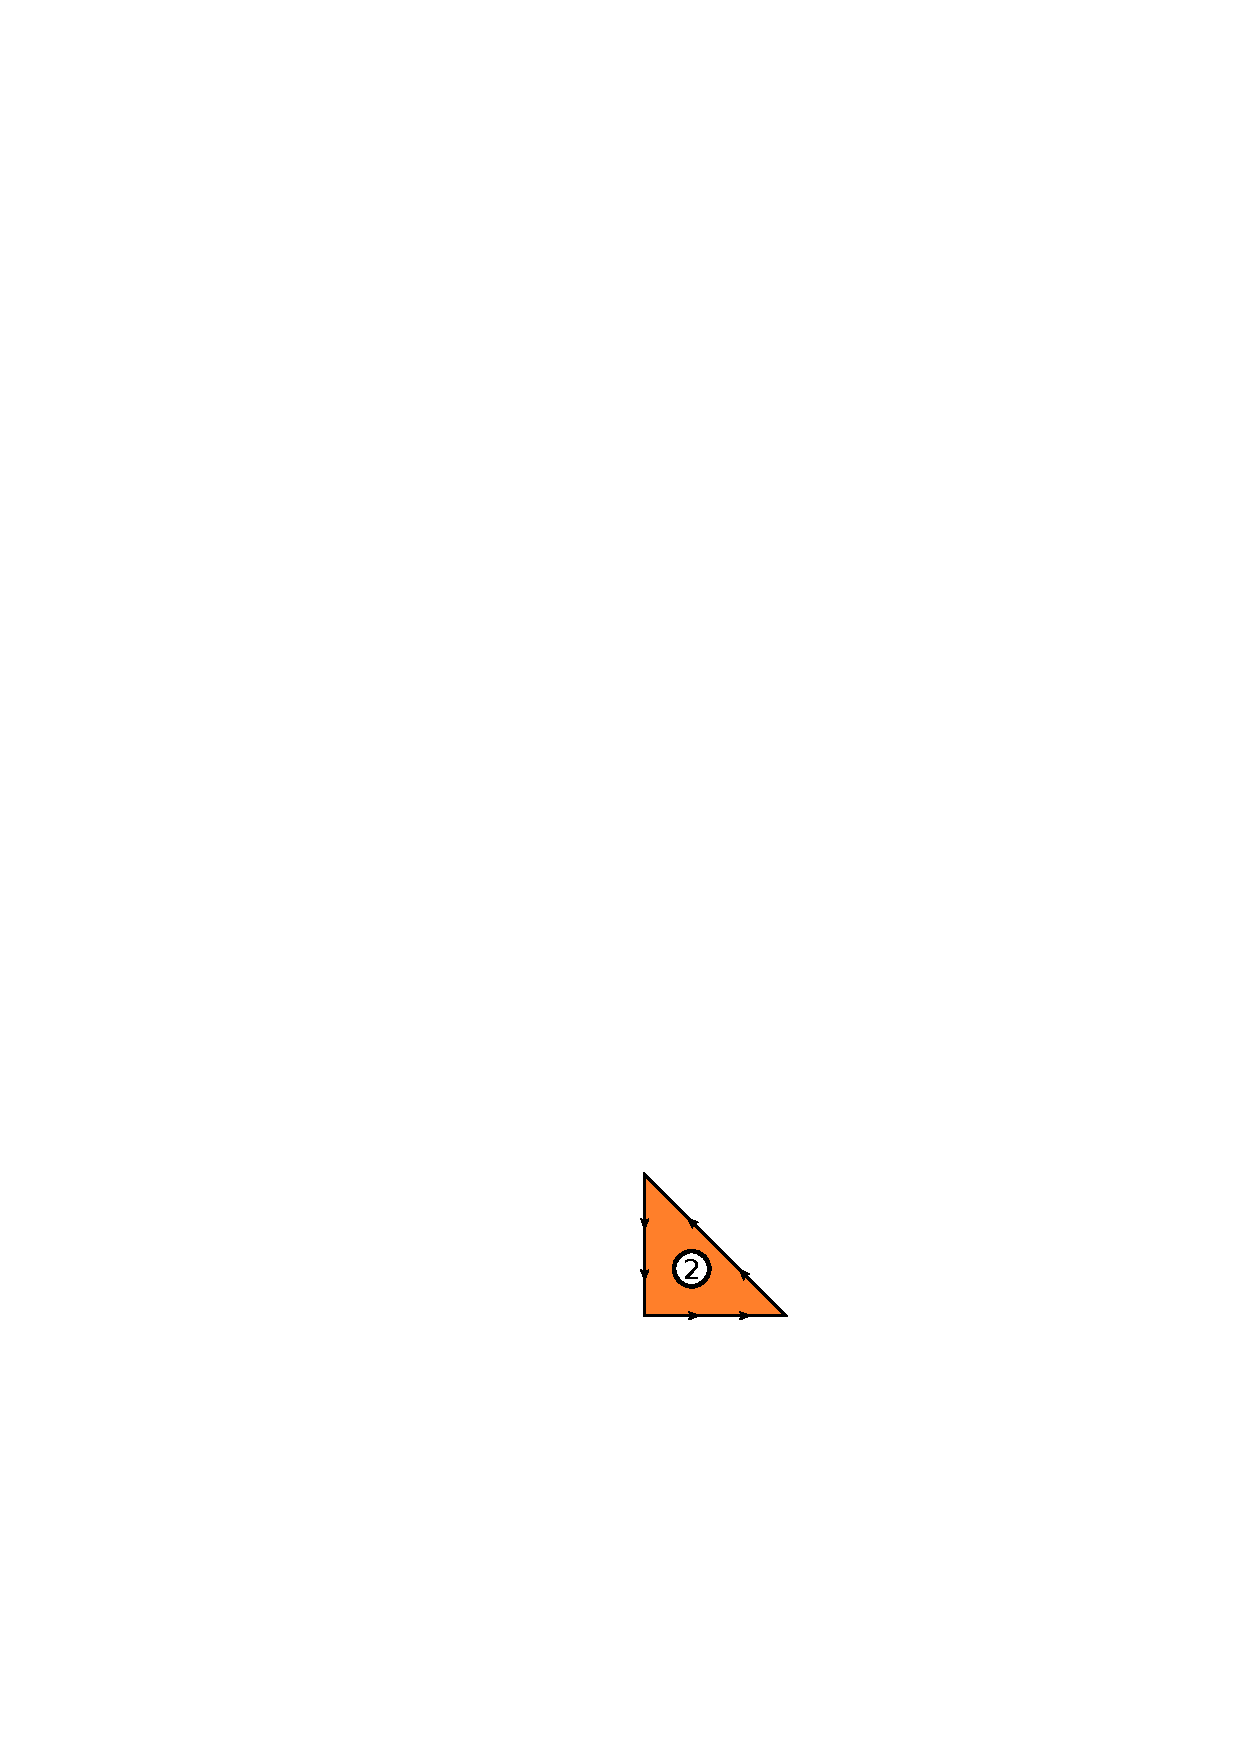
\includegraphics[width=.3\textwidth]{figures/part_4/Ned1.pdf}}
\caption{\label{fig:HcurlFE} $H(curl)$ Finite Elements: (Left)  N\'ed\'elec Element $N_0$ of order 1, (Right)  Brezzi-N\'ed\'elec Element $N_1$ of order 2}
\end{figure}

\begin{remark}
The extension to 3D for tensor product element is also quite natural by considering the components separetely and noticing that in 3D there are two tangential components and three normal components.

Simplex based $H(\textrm{curl}, \Omega)$ Finite Elements, which are constructed on tetrahedra in 3D are fundamentally different from   their $H(\textrm{div}, \Omega)$ counterpart, unlike in 2D where one could go from one to the other by a simple rotation of the components. There are also two classes of finite elements, like Raviart-Thomas and Brezzi-Douglas-Marini in 2D, which are called respectively N\'ed\'elec elements of first type and of second type.

The 3D N\'ed\'elec space in which the elements of first type live and which is used to define the degrees of freedom of the N\'ed\'elec elements of second type reads
\begin{equation}\label{nedelec3D}
N_k= ( \mathbb{P}_k)^3 \oplus \left( \mathbf{x}\times ( \mathbb{P}_k)^3 \right)
\end{equation}
and the degrees of freedom are defined by the following unisolvence lemma
\begin{lemma} Let $K$ be a non degenerate tetrahedron, with faces $(f_i)_{0\leq i \leq 4}$, and edges
$(e_i)_{0\leq i \leq 6}$
$k\geq 0$, and $ \mathbf{p}\in N_k(K)$ then
\begin{align}
\int_{e_i} \mathbf{p}\cdot \ut_i \,r \dd s &=0, \quad \forall r\in \mathbb{P}_k(e_i), \label{eq:Ne3d}\\
\int_{f_i} (\mathbf{p}\times \un_i) \cdot \mathbf{s} \dd s &=0, \quad \forall  \mathbf{s}\in (\mathbb{P}_{k-1}(f_i))^2, \label{eq:Nf1}\\
\int_K \mathbf{p}  \cdot \mathbf{q} \dd \mathbf{x} &=0 \quad\forall \mathbf{q} \in (\mathbb{P}_{k-2})^2
\label{eq:Nt}
\end{align}
implies that $ \mathbf{p}=0$.
\end{lemma}
We denote here by $\ut_i$ the unit vector along the edge $e_i$ and by $ \un_i$ the outward unit normal on face $f_i$.
\end{remark}

\section{Change of local basis}

The local degrees of freedom $\Sigma$ of a Finite Element defined by $(K,P,\Sigma)$ can also be used to compute the element matrices with respect to the matrices corresponding to a simpler or easily computable basis of the same space $P$ of dimension $N$. This could for example be an orthonormal basis.
This allows to compute the matrices once for all in some basis and then to get the matrices in any other basis by just computing the corresponding generalised Vandermode matrix as follows.

Let us denote by $(\phi_l)_{0\leq l\leq N}$ the reference basis in which the element matrices are known. 
Let now $(\hat{p}_j)_{0\leq j\leq N}$ be another basis of the same linear space $P$ associated to the degrees of freedom $(\sigma_i)_{0\leq i\leq N}$.
Then $\hat{p}_j$ can be expressed in the basis $(\phi_l)_{0\leq l\leq N}$:
\begin{equation}\label{eq:pphi}
\hat{p}_j(\mathbf{x}) = \sum_{l=1}^{N} \alpha_{j,l} \phi_l(\mathbf{x}).
\end{equation}
Denoting by $\hat{\mathbf{p}}=(\hat{p}_1,\dots,\hat{p}_{N})^\top$, $\boldsymbol{\phi}=(\phi_1,\dots,\phi_{N})^\top$ and $A=((\alpha_{j,l}))_{1\leq j,l \leq N}$, this relation can be written in matrix form
$$
\hat{\mathbf{p}}(\mathbf{x}) = A \boldsymbol{\phi}(\mathbf{x}).
$$
Applying the linear forms $\sigma_i$ to relation  \eqref{eq:pphi} for $1\leq i\leq N$, we get 
\begin{equation}\label{av}
\mathbb{I}_{N} = VA^\top,
\end{equation}
where $ \mathbb{I}_{N}$ is the identity matrix and $V=((\sigma_i(\phi_j)))_{1\leq i,j \leq N}$. The matrix $V$ is called generalised Vandermonde matrix, as in the case when  $((\phi_j))_{1\leq j \leq N}$ is the monomial basis $(1, x, \dots, x^{N-1})$ of $ \mathbb{P}_k$ in
1D and for a Lagrange Finite Element where $\sigma_i(\hat{p}_j)= \hat{p}_j(x_i)$, the matrix $V$ is the classical Vandermonde matrix $V=((x_i^{j-1}))_{1\leq i,j \leq N}$.

The generalised  Vandermonde matrix $V$ is explicitly  computable when the basis $(\phi_j)_j$ and the degrees of freedom $(\sigma_i)_i$ are explicitly known. 
From relation (\ref{av}), it follows immediately that $A=V^{-\top}$, where we denote by $V^{-\top}$
the inverse of the transpose of $V$.

One can also take the derivative of formula \eqref{eq:pphi}. Thus
$$\partial_{x}\hat{p}_j(\mathbf{x}) = \sum_{l=1}^{N} \alpha_{j,l} \partial_x\phi_l(\mathbf{x}),$$
and the same for the other variables if needed.
Applying again the linear form $\sigma_i$ to this equation for $1\leq i\leq N$,  we find
$$D_x\hat{\mathbf{p}} = D_x\boldsymbol{\phi}A^\top=D_x\boldsymbol{\phi}V^{-1} ,$$
where the matrices $D_x\hat{\mathbf{p}}$ and  $D_x\boldsymbol{\phi}$ are defined respectively
by their generic element $((\sigma_i(\partial_x \hat{p}_j)))_{1\leq i,j \leq N}$ 
and $((\sigma_i(\partial_x \phi_j)))_{1\leq i,j \leq N_k}$. Note that if
$(\phi_j)_j$ has been chosen such $D_x\phi$ is explicitly computable, we can, thanks to this relation explicitly compute the matrix $D_x\hat{\mathbf{p}}$ and similarly the derivative matrices with respect to other variables.

We can express $\hat{M}$ the mass matrix on the reference element  $\hat{K}$ using the Vandermonde matrix $V$. Using formula \eqref{eq:pphi}, 
$$\hat{p}_j(\mathbf{x})=  \sum_{l=1}^{N} \alpha_{j,l} \phi_l(\mathbf{x}).$$
Hence $$\int_{\hat{K}} \hat{p}_i(\mathbf{x})\hat{p}_j(\mathbf{x})\,d\mathbf{x}
=  \sum_{l=1}^{N} \sum_{m=1}^{N}\alpha_{i,l}\alpha_{j,m} \int_{\hat{K}}\phi_l(\mathbf{x})\phi_m(\mathbf{x})\,d\mathbf{x} = \sum_{l=1}^{N}\alpha_{i,l}\alpha_{j,m},$$
if the basis functions $(\phi_j)_j$ are  orthonormal on $\hat{K}$. It follows that
$\hat{M}=AA^\top = V^{-\top}V^{-1}$.

If the space $P$ is stable by derivation,
as is the case for the polynomial space $\mathbb{P}_k$, we can also express the derivative 
 $\partial_x G_h$ or other derivatives in the  basis  
 $(p_i)_i$ and this derivative can also be characterised by the degrees of freedom 
$(\sigma_i(\partial_x G_h))_{1\leq i \leq N_k}$. We denote by $D_x\mathbb{G}$
the vector containing these degrees of freedom, which can be expressed using $\mathbb{G}$
as follows. We have
$$\partial_x G_h(\mathbf{x}) = \sum_{j=1}^{N_k} \sigma_j(G_h)\partial_x p_j(\mathbf{x}),$$
and so for $1\leq i\leq N$,
$$\sigma_i(\partial_x G_h) = \sum_{j=1}^{N_k} \sigma_j(G_h)\sigma_i(\partial_x p_j).$$
This can also be written $D_x\mathbb{G}= (D_x\mathbf{p})\mathbb{G}$,
denoting by $D_x\mathbf{p}$ the matrix with generic term $((\sigma_i(\partial_x p_j)))_{1\leq i,j \leq N}$.

\section{Problems}

\begin{exercise}
  TODO
\end{exercise}
